\documentclass{scrartcl}

%\usepackage{algorithm}
%\usepackage{algorithmic}
\usepackage{amsmath}
\usepackage{amssymb}
%\usepackage{array}
%\usepackage{blindtext}
\usepackage{booktabs}
%\usepackage{colortbl}
%\usepackage{comment}
\usepackage{etex}
%\usepackage{float}
\usepackage[T1]{fontenc}
\usepackage{graphicx}
\usepackage[space]{grffile}
%\usepackage{multirow}
\usepackage[utf8]{inputenc}
\usepackage{pgfplots}
\usepackage{pgfplotstable}
\usepackage{morefloats}
\usepackage{subcaption}
%\usepackage{standalone}
\usepackage{times}
\usepackage{tikz}
%\usepackage{todonotes}
\usepackage{xspace}
\usepackage[breaklinks=true,colorlinks,bookmarks=false]{hyperref} %Hyperref should go last

%float setup
%\newfloat{algorithm}{t}{}
%
%%hyperref setup
\hypersetup{colorlinks=true}
\hypersetup{linktoc=all}
\hypersetup{draft=false}
\hypersetup{urlcolor=blue}
\hypersetup{citecolor=black}
\hypersetup{linkcolor=black}
%
%%tikz setup
%\usetikzlibrary{arrows,calc,external,fit,shapes}
\usetikzlibrary{external}
\tikzexternalize[prefix=ext/]
\tikzexternaldisable
%\usetikzlibrary{backgrounds}
%\usetikzlibrary{pgfplots.groupplots}
%
\pgfplotsset{compat=1.10}
%\pgfplotsset{filter discard warning=false}
%
%%Set graphics path
%\graphicspath{{figures//}}
%
%\DeclareMathOperator*{\argmin}{arg\,min}
%\DeclareMathOperator*{\argmax}{arg\,max}
%
%%Make require and ensure input and output
%\renewcommand{\algorithmicrequire}{\textbf{Input:}}
%\renewcommand{\algorithmicensure}{\textbf{Output:}}
%
%%This can be used to add external file dependencies for latexmk
%\makeatletter
%\newcommand*{\addFileDependency}[1]{% argument=file name and extension
%  \typeout{(#1)}% latexmk will find this if $recorder=0 (however, in that case, it will ignore #1 if it is a .aux or .pdf file etc and it exists! if it doesn't exist, it will appear in the list of dependents regardless)
%  \@addtofilelist{#1}% if you want it to appear in \listfiles, not really necessary and latexmk doesn't use this
%  \IfFileExists{#1}{}{\typeout{No file #1.}}% latexmk will find this message if #1 doesn't exist (yet)
%}
%\makeatother
%
\newcommand{\mytodo}[1]{\textcolor{red}{TODO: #1}}


% Probability of event
% 1st optional parameter: footnote (probability w.r.t. specific random variable / condition)
% 2nd optional parameter: determine the size of the brackes (big, Big, bigg, Bigg, normal), standard: \left, \right
\DeclareDocumentCommand{\Prob}{ O{\empty} O{\empty} m}{
  \ensuremath{
    \mathrm{P}
    \ifthenelse{\equal{#1}{\empty}}{}{_{#1}}
    \ifthenelse{\equal{#2}{big}}{\big\{{#3}\big\}}{
      \ifthenelse{\equal{#2}{Big}}{\Big\{{#3}\Big\}}{
        \ifthenelse{\equal{#2}{bigg}}{\bigg\{{#3}\bigg\}}{
          \ifthenelse{\equal{#2}{Bigg}}{\Bigg\{{#3}\Bigg\}}{
            \ifthenelse{\equal{#2}{normal}}{\{{#3}\}}{\left\{{#3}\right\}}
          }
        }
      }
    }
  }
}

% Expectation
% 1st optional parameter: footnote (expectation w.r.t. specific random variable / condition)
% 2nd optional parameter: determine the size of the brackes (big, Big, bigg, Bigg, normal), standard: \left, \right
\DeclareDocumentCommand{\E}{ O{\empty} O{\empty} m}{
  \ensuremath{
%    \raisebox{-1.5pt}{\ensuremath{\mathlarger{\mathlarger{\mathbbmss{E}}}}}
    \ensuremath{\mathlarger{\mathbbmss{E}}}
    \ifthenelse{\equal{#1}{\empty}}{}{_{#1}}
    \ifthenelse{\equal{#2}{big}}{\big[{#3}\big]}{
      \ifthenelse{\equal{#2}{Big}}{\Big[{#3}\Big]}{
        \ifthenelse{\equal{#2}{bigg}}{\bigg[{#3}\bigg]}{
          \ifthenelse{\equal{#2}{Bigg}}{\Bigg[{#3}\Bigg]}{
            \ifthenelse{\equal{#2}{normal}}{[{#3}]}{\left[{#3}\right]}
          }
        }
      }
    }
  }
}

% Inner product
%  optional parameter: determine the size of the brackes (big, Big, bigg, Bigg, normal), standard: \left, \right
\DeclareDocumentCommand{\inprod}{  O{\empty} m m}{
  \ensuremath{
    \ifthenelse{\equal{#1}{big}}{\big\langle{#2},{#3}\big\rangle}{
      \ifthenelse{\equal{#1}{Big}}{\Big\langle{#2},{#3}\Big\rangle}{
        \ifthenelse{\equal{#1}{bigg}}{\bigg\langle{#2},{#3}\bigg\rangle}{
          \ifthenelse{\equal{#1}{Bigg}}{\Bigg\langle{#2},{#3}\Bigg\rangle}{
            \ifthenelse{\equal{#1}{normal}}{\langle{#2},{#3}\rangle}{\left\langle{#2},{#3}\right\rangle}
          }
        }
      }
    }
  }
}

% Norm
%  optional parameter: determine the size of the brackes (big, Big, bigg, Bigg, normal), standard: \left, \right
\DeclareDocumentCommand{\norm}{  O{\empty} m}{
  \ensuremath{
    \ifthenelse{\equal{#1}{big}}{\big\Vert{#2}\big\Vert}{
      \ifthenelse{\equal{#1}{Big}}{\Big\Vert{#2}\Big\Vert}{
        \ifthenelse{\equal{#1}{bigg}}{\bigg\Vert{#2}\bigg\Vert}{
          \ifthenelse{\equal{#1}{Bigg}}{\Bigg\Vert{#2}\Bigg\Vert}{
            \ifthenelse{\equal{#1}{normal}}{\Vert{#2}\Vert}{\left\Vert{#2}\right\Vert}
          }
        }
      }
    }
  }
}

\newcommand{\sign}{\mathrm{sign}}

\newcommand{\rv}[1]{\mathsf{#1}}  				 %Random Variable. Write them in lower case letters.
\renewcommand{\vec}[1]{\mathbf{#1}}	 %deterministic vector
\newcommand{\rvec}[1]{{\textbf{\textsf{#1}}}}%random vector
\newcommand{\mat}[1]{\uppercase{\mathbf{#1}}}   %deterministic matrix. Use lower case letters, the command makes them uppercase
\newcommand{\rmat}[1]{\uppercase{\textbf{\textsf{#1}}}}   %random matrix. Use lower case letters, the command makes them uppercase

\DeclareMathOperator*{\argmax}{arg\,max}
\DeclareMathOperator*{\argmin}{arg\,min}

\title{Machine Learning SS 2014}
\subtitle{Exercise Sheet 1}

\author{Georg Nebehay\\gnebehay@gmail.com
\and
Michael Meidlinger\\
michael.meidlinger@nt.tuwien.ac.at
}

\date{}

\tikzset{%
level 1/.style={sibling distance=10em},%
level 2/.style={sibling distance=7em},%
level 3/.style={sibling distance=3em}%
}

\begin{document}

\maketitle

\section{Decision Trees}

We modified the algorithm presented in the slides slightly in a sense that
a feature must not be selected in a node when it was already used in a parent node.
The following classification results were obtained:

\begin{center}
  \begin{tabular}{cc}
    \toprule
    Tree & Accuracy\\
    \midrule
    a) & 3/6\\
    b) & 4/6\\
    c) & 2/6\\
    d) & 2/6\\
    \bottomrule
  \end{tabular}
\end{center}

In the following sections, individual decision trees and classification results are given.
Details about each step of the tree construction are in the appendix.

%\begin{table}[h!]
%  \centering
%  \begin{tabular}{cccccc|c}
%    \toprule
%    person      & eyes  & handsome & height & sex    & soccer & date\\
%    \midrule
%    Apu         & blue  & yes      & tall   & male   & no     & yes \\
%    Bernice     & brown & yes      & short  & female & no     & no  \\
%    Carl        & blue  & no       & tall   & male   & no     & yes \\
%    Doris       & green & yes      & short  & female & no     & no  \\
%    Edna        & brown & no       & short  & female & yes    & no  \\
%    Prof. Frink & brown & yes      & tall   & male   & yes    & no  \\
%    Gil         & blue  & no       & tall   & male   & yes    & no  \\
%    Homer       & green & yes      & short  & male   & no     & yes \\
%    Itchy       & brown & no       & short  & male   & yes    & yes \\
%    \bottomrule
%  \end{tabular}
%  \caption{Training data.}
%\end{table}

%\begin{table}[h!]
%  \centering
%  \begin{tabular}{cccccc|c}
%    \toprule
%    person      & eyes  & handsome & height & sex    & soccer & date\\
%    \midrule
%    Jimbo       & blue  & no       & tall   & male   & no     & yes\\
%    Krusty      & green & yes      & short  & male   & yes    & no\\
%    Lisa        & blue  & yes      & tall   & female & no     & no\\
%    Moe         & brown & no       & short  & male   & no     & no\\
%    Ned         & brown & yes      & short  & male   & no     & yes\\
%    Quimby      & blue  & no       & tall   & male   & no     & yes\\
%    \bottomrule
%  \end{tabular}
%  \caption{Test data.}
%\end{table}

\subsection{Without attribute ``soccer''}

At iteration 4, the algorithm enters an infinite recursion.
The problem stems from the omission of the soccer feature,
leading to the two datapoints Carl and Gil sharing exactly the same feature values but opposite labels.
We chose to stop the recursion at this point and to replace the node with the majority output of the parent node.
The decision tree is shown in Figure~\ref{fig:tree-nosoccer}.
Classification results are in~\ref{tab:tree-nosoccer}.

\begin{figure}[h!]
\centering 
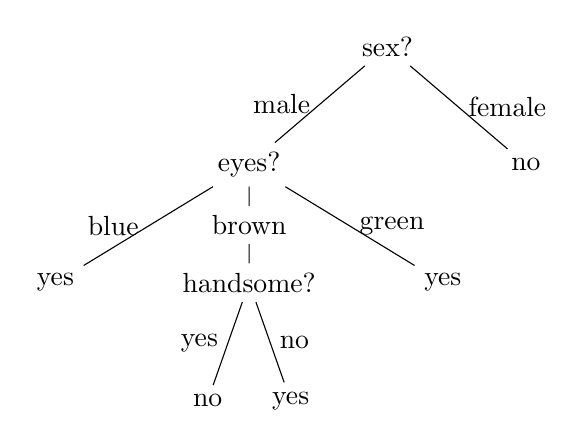
\begin{tikzpicture}
  \node {sex?}
  child { node {eyes?}
    child { node {yes} edge from parent node[left] {blue} }
    child { node {handsome?}
      child { node {no} edge from parent node[left] {yes} }
      child { node {yes} edge from parent node[right] {no} }
      edge from parent node[fill=white] {brown} }
    child { node {yes} edge from parent node[right] {green} }
    edge from parent node[left] {male} }
  child { node {no} 
    edge from parent node[right] {female}
  };
\end{tikzpicture}
\caption{Decision tree for task a)}
\label{fig:tree-nosoccer}
\end{figure}

\begin{table}[h!]
  \centering
  \begin{tabular}{cccccc|c|c}
    \toprule
    person      & eyes  & handsome & height & sex    & soccer & date & tree\\
    \midrule
    Jimbo       & blue  & no       & tall   & male   & no     & yes & yes\\
    Krusty      & green & yes      & short  & male   & yes    & no  & yes\\
    Lisa        & blue  & yes      & tall   & female & no     & no  & no\\
    Moe         & brown & no       & short  & male   & no     & no  & yes\\
    Ned         & brown & yes      & short  & male   & no     & yes & no\\
    Quimby      & blue  & no       & tall   & male   & no     & yes & yes\\
    \bottomrule
  \end{tabular}
  \caption{Classification result for tree a) on the test set. Accuracy is 3/6.}
\label{tab:tree-nosoccer}
\end{table}


\subsection{Without attribute ``eyecolor''}

The decision tree is shown in Figure~\ref{fig:tree-noeyes}.
Classification results are in Table~\ref{tab:tree-noeyes}.

\begin{figure}
\centering 
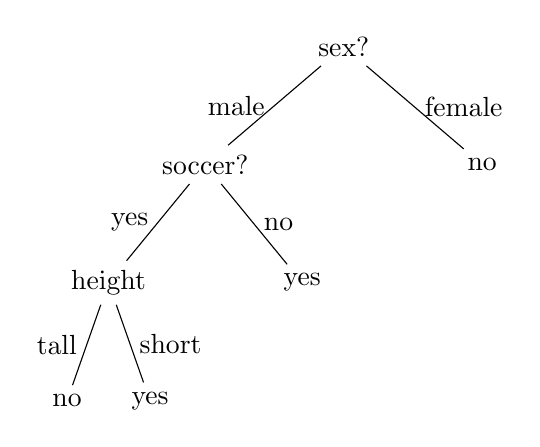
\begin{tikzpicture}
  \node {sex?}
  child { node {soccer?}
    child { node {height}
    child { node {no} edge from parent node[left] {tall} }
    child { node {yes} edge from parent node[right] {short} }
      edge from parent node[left] {yes} }
    child { node {yes} edge from parent node[right] {no} }
    edge from parent node[left] {male} }
  child { node {no} 
    edge from parent node[right] {female}
  };
\end{tikzpicture}
\caption{Decision tree for task b)}
\label{fig:tree-noeyes}
\end{figure}

\begin{table}[h!]
  \centering
  \begin{tabular}{cccccc|c|c}
    \toprule
    person      & eyes  & handsome & height & sex    & soccer & date & tree\\
    \midrule
    Jimbo       & blue  & no       & tall   & male   & no     & yes & yes\\
    Krusty      & green & yes      & short  & male   & yes    & no  & yes\\
    Lisa        & blue  & yes      & tall   & female & no     & no  & no \\
    Moe         & brown & no       & short  & male   & no     & no  & yes\\
    Ned         & brown & yes      & short  & male   & no     & yes & yes\\
    Quimby      & blue  & no       & tall   & male   & no     & yes & yes\\
    \bottomrule
  \end{tabular}
  \caption{Classification result for tree b) on the test set. Accuracy is 4/6.}
  \label{tab:tree-noeyes}
\end{table}

\subsection{Itchy has label ``no''}

The decision tree is shown in Figure~\ref{fig:tree-itchyno}.
Classification results are in Table~\ref{tab:tree-itchyno}.

\begin{figure}
\centering 
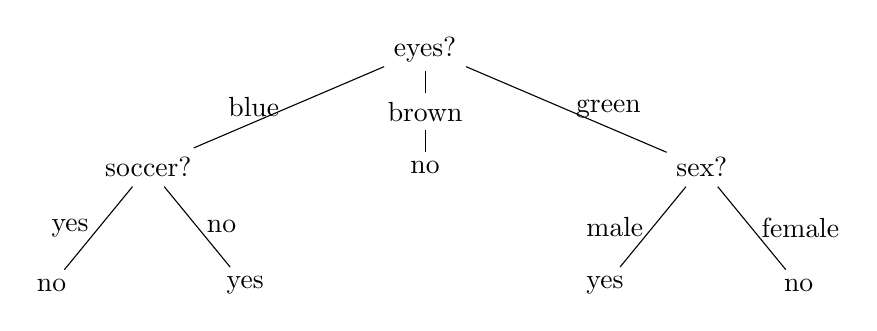
\begin{tikzpicture}
\node {eyes?}
  child { node {soccer?}
    child { node {no} edge from parent node[left] {yes} }
    child { node {yes} edge from parent node[right] {no} }
    edge from parent node[left] {blue} }
  child { node {no} edge from parent node[fill=white] {brown} }
  child { node {sex?}
    child { node {yes} edge from parent node[left] {male} }
    child { node {no} edge from parent node[right] {female} }
  edge from parent node[right] {green} }
;
\end{tikzpicture}
\caption{Decision tree for task c)}
\label{fig:tree-itchyno}
\end{figure}

\begin{table}[h!]
  \centering
  \begin{tabular}{cccccc|c|c}
    \toprule
    person      & eyes  & handsome & height & sex    & soccer & date & tree\\
    \midrule
    Jimbo       & blue  & no       & tall   & male   & no     & yes & no \\
    Krusty      & green & yes      & short  & male   & yes    & no  & yes\\
    Lisa        & blue  & yes      & tall   & female & no     & no  & yes\\
    Moe         & brown & no       & short  & male   & no     & no  & no \\
    Ned         & brown & yes      & short  & male   & no     & yes & no \\
    Quimby      & blue  & no       & tall   & male   & no     & yes & yes\\
    \bottomrule
  \end{tabular}
  \caption{Classification result for tree c) on the test set. Accuracy is 2/6.}
  \label{tab:tree-itchyno}
\end{table}

\subsection{Additional training example ``Ralph''}

The decision tree is shown in Figure~\ref{fig:tree-ralph}.
Classification results are in Table~\ref{tab:tree-ralph}.

\begin{figure}
\centering 
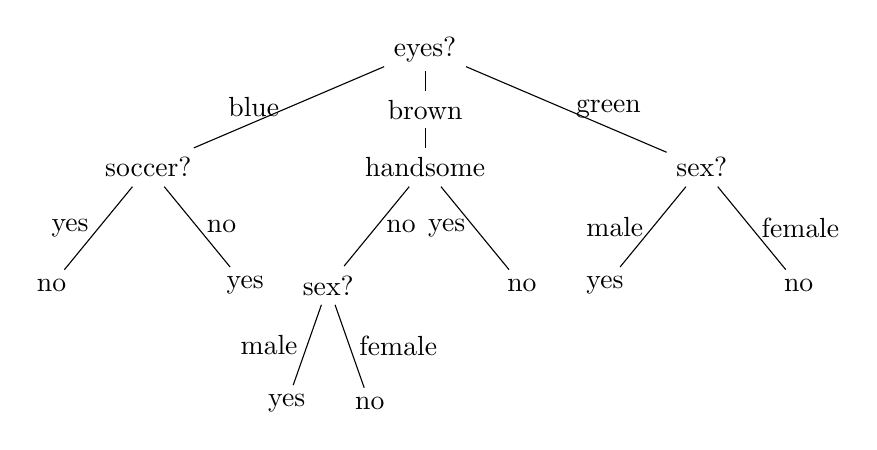
\begin{tikzpicture}
\node {eyes?}
  child { node {soccer?}
    child { node {no} edge from parent node[left] {yes} }
    child { node {yes} edge from parent node[right] {no} }
    edge from parent node[left] {blue} }
  child { node {handsome}
    child { node {sex?}
      child { node {yes} edge from parent node[left] {male} }
      child { node {no} edge from parent node[right] {female} }
      edge from parent node[right] {no} }
    child { node {no} edge from parent node[left] {yes} }
    edge from parent node[fill=white] {brown} }
  child { node {sex?}
    child { node {yes} edge from parent node[left] {male} }
    child { node {no} edge from parent node[right] {female} }
    edge from parent node[right] {green} }
;
\end{tikzpicture}
\caption{Decision tree for task d)}
\label{fig:tree-ralph}
\end{figure}

\begin{table}[h!]
  \centering
  \begin{tabular}{cccccc|c|c}
    \toprule
    person      & eyes  & handsome & height & sex    & soccer & date & tree\\
    \midrule
    Jimbo       & blue  & no       & tall   & male   & no     & yes & yes\\
    Krusty      & green & yes      & short  & male   & yes    & no  & yes\\
    Lisa        & blue  & yes      & tall   & female & no     & no  & yes\\
    Moe         & brown & no       & short  & male   & no     & no  & yes\\
    Ned         & brown & yes      & short  & male   & no     & yes & no \\
    Quimby      & blue  & no       & tall   & male   & no     & yes & yes\\
    \bottomrule
  \end{tabular}
  \caption{Classification result for tree d) on the test set. Accuracy is 2/6.}
  \label{tab:tree-ralph}
\end{table}



\subsection{Additional Attributes}
There are $K=5$ attributes given, none of which a single split along any of those would achieve zero error probability. In order to achieve zero error probability with a single split along any of the $D$ additional attributes, at least one set of values of those must be isomorphic to the dating decision. Let $\vec d \in \lbrace 0,1\rbrace^n$ denote the dating decisions of the $n$ candidates and $\rvec a_i \sim \frac{1}{2^n}$, $i=1,\dots,D$  random vectors representing the additional attributes. We can then derive the probability of zero error with a single split (event $\mathcal A$) as follows:

\begin{align}
	\Prob{\mathcal A}& = 
	\Prob{ \Big(\rvec a_1 = \vec d \vee \rvec a_1 = \neg \vec d \Big) \vee 
		\dots \vee \Big(\rvec a_D = \vec d \vee \rvec a_D = \neg \vec d \Big)} \\
	&= \sum_{i=1}^{D}  \left( \frac{2}{2^n} \right)^i  \left( 1-\frac{2}{2^n}\right)^{D-i} 
	= 1- \left( 1-2^{n-1} \right)^{D} 
	= \begin{cases} 0.0384 &D=10 \\  0.3293 &D=100 \\ 0.9950 &D=1353\end{cases}
\end{align}

\section{Nearest Neighbour Classification}\label{prob2}
\section{Capacity \& Overfitting}
\subsection{Capacity}
We assume consistency of our training data: 
\begin{equation}
	(x^1,y^1),(x^2,y^2)\in \mathcal D: x^1=x^2 \Rightarrow y^1 =y^2.
\end{equation}
\begin{description}
	\item[Decision trees] If we use binary splits $\llbracket x_k \geq \theta_k\rrbracket$, $k=1,\dots,d$ we partition $\mathbb R^2$ into rectangular areas around the training data. If the data is consistent, we can make this partition arbitrarily granular and hence the memory is $\infty$.
	\item[1-NN] is always error free on the training data (cf. problem \ref{prob2}), thus we again have memory $\infty$.
	\item[$K$-NN] has capacity 2, since there is always the possibility that one sample with label $y^1$ is surrounded by $n-1$ samples with label $y^2$.
	\item[Perceptron] The decision $h(x) = \sign(\inprod{w}{x} -\theta)$ corresponds to a hyperplane decision boundary, where the hyperplane is determined by the weight vector $w$ and the offset $\theta$. Thus, to be error free on the training data, it has to be linearly separable, which is guaranteed for $n=2$ or less samples but not for 3 or more arbitrary samples (Imagine 3 samples that can be connected with a line:
	\begin{center}
		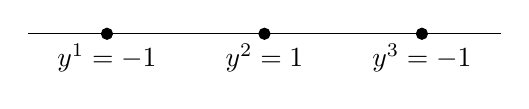
\begin{tikzpicture}
			\draw[fill=black] (0,0) circle [radius=2pt] node[below]{$y^1=-1$};
			\draw[fill=black]  (2,0) circle [radius=2pt] node[below]{$y^2=1$};
			\draw[fill=black]  (4,0) circle [radius=2pt] node[below]{$y^3=-1$};
			\draw (-1,0)--(5,0);
					\end{tikzpicture}
	\end{center}
	\item[Boosting] For this case, the memory depends on the simple component decision rules. In case of the binary coordinate splits that were used in the lecture slides, the situation is similar to the one of the decision tree. Therefore, the memory is $\infty$.
\end{description}
	
	\subsection{Overfitting}
	A high capacity obviously implies overfitting while a low one corresponds to unterfitting. 
	\subsection{Free parameters of the preceptron}
	In $\mathbb R^2$, there are $2$ weight vector elements and the offset $\theta$, thus in total $3$ parameters.
	\subsection{Free parameters of a tree with $L$ leaves}
	Each tree node checks $\llbracket x_k \geq \theta_k\rrbracket$, $k=1,\dots,d$ and hence contributes one parameter $\theta_i$. Consequently, the question reduces to finding the number $I$ of interior nodes of a full, binary tree with $L$ leaves. It can be shown that $I=L-1$ and therefore $L-1$ free parameters.
	
\section{Missing Proofs}
\subsection{Bayes Classifier}
The optimal classifier is given by
\begin{equation}
	c^\star(x) = \argmax_{y \in \mathcal Y} p(y| x) = \argmax_{y \in \mathcal Y} p(x,y),
\end{equation}
which for the binary case $y\in\lbrace -1,1\rbrace$ simplifies to
\begin{equation}
	c^\star(x) = \begin{cases} +1 &  p(+1|x) > p(-1|x) \\ -1 &\text{otherwise}\end{cases} 
	=  \sign \left( \log  \frac{p(+1|x)}{p(-1|x)}\right)
	=  \sign \left( \log  \frac{p(x,+1)}{p(x,-1)}\right),
\end{equation}
since $p(x,y)=p(y|x)p(x)$. \hfill $\blacksquare$

In communications, the quantities $\log  \frac{p(+1|x)}{p(-1|x)}$ are referred to as \emph{Log-Likelihood-Ratios (LLRs)} and are used in iterative decoding algorithms to quantify wether a bit was $+1$ or $-1$, given the received signal $x$.

\subsection{Minimum Risk Classifier}
The optimal classifier is given by
\begin{equation}
	c_\ell^\star(x) = \argmin_{y \in \mathcal Y}\E[\overline y \sim p(\overline y | x)][]{\ell(\overline y, y)}
					=  \argmin_{y \in \mathcal Y} \sum_{\overline y \in \mathcal Y} p(\overline y | x) \ell(\overline y, y) ,
\end{equation}
which for the binary case $y\in\lbrace -1,1\rbrace$ simplifies to
\begin{equation}
	c_\ell^\star(x) = \begin{cases} +1 &  p(+1|x)\underbrace{\ell(+1,+1)}_{d} + p(-1|x)\underbrace{\ell(-1,+1)}_{b} <
															p(+1|x)\underbrace{\ell(+1,-1)}_{c} + p(-1|x)\underbrace{\ell(-1,-1)}_{a} \\ 
													-1 &\text{otherwise}\end{cases} 
\end{equation}
and hence
\begin{equation}
	c_\ell^\star(x) =  \sign \left( \log  \frac{p(+1|x)(c-d)}{p(-1|x)(b-a)}\right) 
							= \sign \left( \log  \frac{p(+1|x)}{p(-1|x)} + \log{\frac{c-d}{b-a}}\right). \hfill \blacksquare
\end{equation}
\section{Practical Experiments I}
\subsection{Decision Trees}
\begin{tikzpicture}
  \begin{axis}[
    xlabel=Complexity (\# of interior nodes),
    ylabel=Error,
    title=normal run]
	\addplot table[ header=false] {tree_continous/5a1_train.txt};%
	\addplot table[header=false] {tree_continous/5a1_test.txt};%};%
    \addlegendentry{training}%
    \addlegendentry{testing}%
  \end{axis}
\end{tikzpicture}
\begin{tikzpicture}
  \begin{axis}[
    xlabel=Complexity (\# of interior nodes),
    ylabel=Error,
    title=switched label of $y^9$]
	\addplot table[ header=false] {tree_continous/5a2_train.txt};%
	\addplot table[header=false] {tree_continous/5a2_test.txt};%};%
    \addlegendentry{training}%
    \addlegendentry{testing}%
  \end{axis}
\end{tikzpicture}



\subsection{$k$-Nearest-Neighbor}
\begin{tikzpicture}
  \begin{axis}[
    xlabel=Complexity ($k$),
    ylabel=Error,
    title=normal run]
	\addplot table[ header=false] {knn/5b1_train.txt};%
	\addplot table[header=false] {knn/5b1_test.txt};%};%
    \addlegendentry{training}%
    \addlegendentry{testing}%
  \end{axis}
\end{tikzpicture}
\begin{tikzpicture}
  \begin{axis}[
    xlabel=Complexity ($k$),
    ylabel=Error,
    title=switched label of $y^9$]
	\addplot table[ header=false] {knn/5b2_train.txt};%
	\addplot table[header=false] {knn/5b2_test.txt};%};%
    \addlegendentry{training}%
    \addlegendentry{testing}%
  \end{axis}
\end{tikzpicture}


\subsection{Perceptron}

\begin{tikzpicture}
  \begin{axis}[
    xlabel=Complexity,
    ylabel=Error,
  title=normal run]
    \addplot table[x expr=\coordindex,y index=0, header=false] {artificial1-trainerror-perc.txt};%
    \addplot table[x expr=\coordindex,y index=0, header=false] {artificial1-testerror-perc.txt};%
    \addlegendentry{training}%
    \addlegendentry{testing}%
  \end{axis}
  
\end{tikzpicture}
\begin{tikzpicture}
  \begin{axis}[
    xlabel=Complexity,
    ylabel=Error,
	mark repeat = 10,
  title=switched label of $y^9$]
	\addplot table[x expr=\coordindex,y index=0, header=false] {artificial2-trainerror-perc.txt};%
	\addplot table[x expr=\coordindex,y index=0, header=false] {artificial2-testerror-perc.txt};%
    \addlegendentry{training}%
    \addlegendentry{testing}%
  \end{axis}
  
\end{tikzpicture}

\subsection{AdaBoost}

\begin{tikzpicture}
  \begin{axis}[
    xlabel=Complexity,
    ylabel=Error,
  title=normal run]
	\addplot table[x expr=\coordindex,y index=0, header=false] {artificial1-trainerror-boost.txt};%
	\addplot table[x expr=\coordindex,y index=0, header=false] {artificial1-testerror-boost.txt};%
    \addlegendentry{training}%
    \addlegendentry{testing}%
  \end{axis}
  
\end{tikzpicture}
\begin{tikzpicture}
  \begin{axis}[
    xlabel=Complexity,
    ylabel=Error,
  title=switched label of $y^9$]
	\addplot table[x expr=\coordindex,y index=0, header=false] {artificial2-trainerror-boost.txt};%
	\addplot table[x expr=\coordindex,y index=0, header=false] {artificial2-testerror-boost.txt};%
    \addlegendentry{training}%
    \addlegendentry{testing}%
  \end{axis}
  
\end{tikzpicture}

\section{Practical Experiments II}
\subsection{AdaBoost}
In order to perform multiclass classification on the wine dataset using AdaBoost,
we employed a one-versus-all strategy.
We trained one classifier for each class,
using examples from one class as positive examples and
examples from all other classes as negative examples.
We combined the classifiers by predicting the label $y$ for which the corresponding classifier
reports the highest confidence score
%
\begin{equation}
  \hat y = \argmax_{k \in 1 \ldots K} f_k(x)  
\end{equation}
%
Using this method we achieve a test error of $E=8$ on the wine dataset.


\subsection{Decision Tree}
\begin{tikzpicture}
  \begin{axis}[
    xlabel=Complexity (\# of interior nodes),
    ylabel=Error]
	\addplot table[ header=false] {tree_continous/6a_train.txt};%
	\addplot table[header=false] {tree_continous/6a_test.txt};%};%
    \addlegendentry{training}%
    \addlegendentry{testing}%
  \end{axis}
\end{tikzpicture}

\subsection{$k$-Nearest-Neighbor}
Here we have the problem that the different properties have a very different scaling. For large $k$, underfitting causes high error rates.

\begin{tikzpicture}
  \begin{axis}[
    xlabel=Complexity ($k$),
    ylabel=Error,
    legend pos=north west]
	\addplot table[ header=false] {knn/6b_train.txt};%
	\addplot table[header=false] {knn/6b_test.txt};%};%
    \addlegendentry{training}%
    \addlegendentry{testing}%
  \end{axis}
\end{tikzpicture}

\clearpage

\section{Appendix}

\begin{table}[h!]
  \centering
  \begin{tabular}{ccccc|c}
    \toprule
    person      & eyes  & handsome & height & sex    & date\\
    \midrule
    Apu         & blue  & yes      & tall   & male   & yes \\
    Bernice     & brown & yes      & short  & female & no  \\
    Carl        & blue  & no       & tall   & male   & yes \\
    Doris       & green & yes      & short  & female & no  \\
    Edna        & brown & no       & short  & female & no  \\
    Prof. Frink & brown & yes      & tall   & male   & no  \\
    Gil         & blue  & no       & tall   & male   & no  \\
    Homer       & green & yes      & short  & male   & yes \\
    Itchy       & brown & no       & short  & male   & yes \\
    \bottomrule
  \end{tabular}

  \vspace{.5cm}

  \begin{tabular}{ccc}
    \toprule
    Feature      & Accuracies                              & Total\\
    \midrule
    eyes         & blue: (2/3), brown: (3/4), green: (1/2) & 6/9\\
    handsome     & yes: (3/5), no: (2/4)                   & 5/9\\
    height       & tall: (2/4), short: (3/5)               & 5/9\\
    \textbf{sex} & male: (4/6), female: (3/3) [no]         & \textbf{7/9}\\
    \bottomrule
  \end{tabular}
  \caption*{No soccer, iteration 1, root branch. Best feature: sex}
\end{table}

\begin{table}[h!]
  \centering
  \begin{tabular}{ccccc|c}
    \toprule
    person      & eyes  & handsome & height & sex    & date\\
    \midrule
    Apu         & blue  & yes      & tall   & male   & yes \\
    Carl        & blue  & no       & tall   & male   & yes \\
    Prof. Frink & brown & yes      & tall   & male   & no  \\
    Gil         & blue  & no       & tall   & male   & no  \\
    Homer       & green & yes      & short  & male   & yes \\
    Itchy       & brown & no       & short  & male   & yes \\
    \bottomrule
  \end{tabular}

  \vspace{.5cm}

  \begin{tabular}{ccc}
    \toprule
    Feature       & Accuracies                                    & Total\\
    \midrule
    \textbf{eyes} & blue: (2/3), brown: (1/2), green: (1/1) [yes] & 4/6\\
    handsome      & yes: (2/3), no: (2/3)                         & 4/6\\
    height        & tall: (2/4), short: (2/2)                     & 4/6\\
    sex           & male: (4/6)                                   & 4/6\\
    \bottomrule
  \end{tabular}
  \caption*{No soccer, iteration 2, sex=male branch. Best feature: eyes}
\end{table}

\begin{table}[h!]
  \centering
  \begin{tabular}{ccccc|c}
    \toprule
    person      & eyes  & handsome & height & sex    & date\\
    \midrule
    Apu         & blue  & yes      & tall   & male   & yes \\
    Carl        & blue  & no       & tall   & male   & yes \\
    Gil         & blue  & no       & tall   & male   & no  \\
    \bottomrule
  \end{tabular}

  \vspace{.5cm}

  \begin{tabular}{ccc}
    \toprule
    Feature           & Accuracies                  & Total\\
    \midrule
    eyes              & blue: (2/3)                 & \textbf{2/3}\\
    \textbf{handsome} & yes: (1/1) [yes], no: (1/2) & \textbf{2/3}\\
    height            & tall: (2/3)                 & \textbf{2/3}\\
    sex               & male: (2/3)                 & \textbf{2/3}\\
    \bottomrule
  \end{tabular}
  \caption*{No soccer, iteration 3, sex=male,eyes/blue branch. Best feature: handsome}
\end{table}

\begin{table}[h!]
  \centering
  \begin{tabular}{ccccc|c}
    \toprule
    person      & eyes  & handsome & height & sex    & date\\
    \midrule
    Carl        & blue  & no       & tall   & male   & yes \\
    Gil         & blue  & no       & tall   & male   & no  \\
    \bottomrule
  \end{tabular}

  \vspace{.5cm}

  \begin{tabular}{ccc}
    \toprule
    Feature           & Accuracies                  & Total\\
    \midrule
    eyes              & blue: (1/2)                 & 1/2\\
    handsome          & no: (1/2)                   & 1/2\\
    height            & tall: (1/2)                 & 1/2\\
    sex               & male: (1/2)                 & 1/2\\
    \bottomrule
  \end{tabular}
  \caption*{No soccer, iteration 4, sex=male,eyes/blue,handsome=no branch.
  Stopping because of infinite recursion that lies ahead.}
\end{table}

\begin{table}[h!]
  \centering
  \begin{tabular}{ccccc|c}
    \toprule
    person      & eyes  & handsome & height & sex    & date\\
    \midrule
    Prof. Frink & brown & yes      & tall   & male   & no  \\
    Itchy       & brown & no       & short  & male   & yes \\
    \bottomrule
  \end{tabular}

  \vspace{.5cm}

  \begin{tabular}{ccc}
    \toprule
    Feature           & Accuracies                              & Total\\
    \midrule
    eyes              & brown: (1/2)                            & 1/2\\
    \textbf{handsome} & yes: (1/1) [no], no: (1/1) [yes]        & \textbf{2/2}\\
    height            & tall: (1/1), short: (1/1)               & \textbf{2/2}\\
    sex               & male: (1/2)                             & 1/2\\
    \bottomrule
  \end{tabular}
  \caption*{No soccer, iteration 5, sex=male,eyes=brown branch. Best feature: handsome}
\end{table}


\begin{table}[h!]
  \centering
  \begin{tabular}{ccccc|c}
    \toprule
    person      & handsome & height & sex    & soccer & date\\
    \midrule
    Apu         & yes      & tall   & male   & no     & yes \\
    Bernice     & yes      & short  & female & no     & no  \\
    Carl        & no       & tall   & male   & no     & yes \\
    Doris       & yes      & short  & female & no     & no  \\
    Edna        & no       & short  & female & yes    & no  \\
    Prof. Frink & yes      & tall   & male   & yes    & no  \\
    Gil         & no       & tall   & male   & yes    & no  \\
    Homer       & yes      & short  & male   & no     & yes \\
    Itchy       & no       & short  & male   & yes    & yes \\
    \bottomrule
  \end{tabular}

  \vspace{.5cm}

  \begin{tabular}{ccc}
    \toprule
    Feature      & Accuracies                              & Total\\
    \midrule
    handsome     & yes: (3/5), no: (2/4)                   & 5/9\\
    height       & tall: (2/4), short: (3/5)               & 5/9\\
    \textbf{sex} & male: (4/6), female: (3/3) [no]         & \textbf{7/9}\\
    soccer       & yes: (3/4), no: (3/5)                   & 6/9\\
    \bottomrule
  \end{tabular}
  \caption*{No eyes, iteration 1, root branch. Best feature: sex}
\end{table}

\begin{table}[h!]
  \centering
  \begin{tabular}{ccccc|c}
    \toprule
    person      & handsome & height & sex    & soccer & date\\
    \midrule
    Apu         & yes      & tall   & male   & no     & yes \\
    Carl        & no       & tall   & male   & no     & yes \\
    Prof. Frink & yes      & tall   & male   & yes    & no  \\
    Gil         & no       & tall   & male   & yes    & no  \\
    Homer       & yes      & short  & male   & no     & yes \\
    Itchy       & no       & short  & male   & yes    & yes \\
    \bottomrule
  \end{tabular}

  \vspace{.5cm}

  \begin{tabular}{ccc}
    \toprule
    Feature         & Accuracies                              & Total\\
    \midrule
    handsome        & yes: (2/3), no: (2/3)                   & 4/6\\
    height          & tall: (2/4), short: (2/2)               & 4/6\\
    sex             & male: (4/6)                             & 4/6\\
    \textbf{soccer} & yes: (2/3), no: (3/3) [yes]             & \textbf{5/6}\\
    \bottomrule
  \end{tabular}
  \caption*{No eyes, iteration 2, sex/male branch. Best feature: soccer}
\end{table}

\begin{table}[h!]
  \centering
  \begin{tabular}{ccccc|c}
    \toprule
    person      & handsome & height & sex    & soccer & date\\
    \midrule
    Prof. Frink & yes      & tall   & male   & yes    & no  \\
    Gil         & no       & tall   & male   & yes    & no  \\
    Itchy       & no       & short  & male   & yes    & yes \\
    \bottomrule
  \end{tabular}

  \vspace{.5cm}

  \begin{tabular}{ccc}
    \toprule
    Feature         & Accuracies                              & Total\\
    \midrule
    handsome        & yes: (1/1), no: (1/2)                   & 2/3\\
    \textbf{height} & tall: (2/2) [no], short: (1/1) [yes]    & \textbf{3/3}\\
    sex             & male: (2/3)                             & 2/3\\
    soccer          & yes: (2/3)                              & 2/3\\
    \bottomrule
  \end{tabular}
  \caption*{No eyes, iteration 3, soccer/yes branch. Best feature: height}
\end{table}

\begin{table}[h!]
  \centering
  \begin{tabular}{cccccc|c}
    \toprule
    person      & eyes  & handsome & height & sex    & soccer & date\\
    \midrule
    Apu         & blue  & yes      & tall   & male   & no     & yes \\
    Bernice     & brown & yes      & short  & female & no     & no  \\
    Carl        & blue  & no       & tall   & male   & no     & yes \\
    Doris       & green & yes      & short  & female & no     & no  \\
    Edna        & brown & no       & short  & female & yes    & no  \\
    Prof. Frink & brown & yes      & tall   & male   & yes    & no  \\
    Gil         & blue  & no       & tall   & male   & yes    & no  \\
    Homer       & green & yes      & short  & male   & no     & yes \\
    Itchy       & brown & no       & short  & male   & yes    & no  \\
    \bottomrule
  \end{tabular}

  \vspace{.5cm}

  \begin{tabular}{ccc}
    \toprule
    Feature      & Accuracies                                    & Total\\
    \midrule
    \textbf{eyes} & blue: (2/3), brown: (4/4) [no], green: (1/2) & \textbf{7/9}\\
    handsome      & yes: (3/5), no: (3/4)                        & 6/9\\
    height        & tall: (2/4), short: (4/5)                    & 6/9\\
    sex           & male: (3/6), female: (3/3)                   & 6/9\\
    soccer        & yes: (4/4), no: (3/5)                        & \textbf{7/9}\\
    \bottomrule
  \end{tabular}
  \caption*{Itchy no, iteration 1, root branch. Best feature: eyes}
\end{table}

\begin{table}[h!]
  \centering
  \begin{tabular}{cccccc|c}
    \toprule
    person      & eyes  & handsome & height & sex    & soccer & date\\
    \midrule
    Apu         & blue  & yes      & tall   & male   & no     & yes \\
    Carl        & blue  & no       & tall   & male   & no     & yes \\
    Gil         & blue  & no       & tall   & male   & yes    & no  \\
    \bottomrule
  \end{tabular}

  \vspace{.5cm}

  \begin{tabular}{ccc}
    \toprule
    Feature         & Accuracies                              & Total\\
    \midrule
    eyes            & blue: (2/3)                             & 2/3\\
    handsome        & yes: (1/1), no: (1/2)                   & 2/3\\
    height          & tall: (2/3)                             & 2/3\\
    sex             & male: (2/3)                             & 2/3\\
    \textbf{soccer} & yes: (1/1) [no], no: (2/2) [yes]        & \textbf{3/3}\\
    \bottomrule
  \end{tabular}
  \caption*{Itchy no, iteration 2, eyes=blue branch. Best feature: soccer}
\end{table}

\begin{table}[h!]
  \centering
  \begin{tabular}{cccccc|c}
    \toprule
    person      & eyes  & handsome & height & sex    & soccer & date\\
    \midrule
    Doris       & green & yes      & short  & female & no     & no  \\
    Homer       & green & yes      & short  & male   & no     & yes \\
    \bottomrule
  \end{tabular}

  \vspace{.5cm}

  \begin{tabular}{ccc}
    \toprule
    Feature      & Accuracies                              & Total\\
    \midrule
    eyes         & green: (1/2)                            & 1/2\\
    handsome     & yes: (1/2)                              & 1/2\\
    height       & short: (1/2)                            & 1/2\\
    \textbf{sex} & male: (1/1) [yes], female: (1/1) [no]   & \textbf{2/2}\\
    soccer       & no: (1/2)                               & 7/9\\
    \bottomrule
  \end{tabular}
  \caption*{Itchy no, iteration 3, eyes=green branch. Best feature: sex}
\end{table}

\begin{table}[h!]
  \centering
  \begin{tabular}{cccccc|c}
    \toprule
    person      & eyes  & handsome & height & sex    & soccer & date\\
    \midrule
    Apu         & blue  & yes      & tall   & male   & no     & yes \\
    Bernice     & brown & yes      & short  & female & no     & no  \\
    Carl        & blue  & no       & tall   & male   & no     & yes \\
    Doris       & green & yes      & short  & female & no     & no  \\
    Edna        & brown & no       & short  & female & yes    & no  \\
    Prof. Frink & brown & yes      & tall   & male   & yes    & no  \\
    Gil         & blue  & no       & tall   & male   & yes    & no  \\
    Homer       & green & yes      & short  & male   & no     & yes \\
    Itchy       & brown & no       & short  & male   & yes    & yes \\
    Ralph       & green & no       & short  & male   & yes    & no  \\
    \bottomrule
  \end{tabular}

  \vspace{.5cm}

  \begin{tabular}{ccc}
    \toprule
    Feature         & Accuracies                              & Total\\
    \midrule
    \textbf{eyes}   & blue: (2/3), brown: (3/4), green: (2/3) & \textbf{7/10}\\
    handsome        & yes: (3/5), no: (3/5)                   & 6/10\\
    height          & tall: (2/4), short: (4/6)               & 6/10\\
    sex             & male: (4/7), female: (3/3)              & \textbf{7/10}\\
    soccer          & yes: (4/5), no: (3/5)                   & \textbf{7/10}\\
    \bottomrule
  \end{tabular}
  \caption*{Ralph, iteration 1, root branch. Best feature: eyes}
\end{table}

\begin{table}[h!]
  \centering
  \begin{tabular}{cccccc|c}
    \toprule
    person      & eyes  & handsome & height & sex    & soccer & date\\
    \midrule
    Apu         & blue  & yes      & tall   & male   & no     & yes \\
    Carl        & blue  & no       & tall   & male   & no     & yes \\
    Gil         & blue  & no       & tall   & male   & yes    & no  \\
    \bottomrule
  \end{tabular}

  \vspace{.5cm}

  \begin{tabular}{ccc}
    \toprule
    Feature         & Accuracies                              & Total\\
    \midrule
    eyes            & blue: (2/3)                             & 2/3\\
    handsome        & yes: (1/1), no: (1/2)                   & 2/3\\
    height          & tall: (2/3)                             & 2/3\\
    sex             & male: (2/3)                             & 2/3\\
    \textbf{soccer} & yes: (1/1) [no], no: (2/2) [yes]        & \textbf{3/3}\\
    \bottomrule
  \end{tabular}
  \caption*{Ralph, iteration 2, eyes=blue branch. Best feature: soccer}
\end{table}

\begin{table}[h!]
  \centering
  \begin{tabular}{cccccc|c}
    \toprule
    person      & eyes  & handsome & height & sex    & soccer & date\\
    \midrule
    Bernice     & brown & yes      & short  & female & no     & no  \\
    Edna        & brown & no       & short  & female & yes    & no  \\
    Prof. Frink & brown & yes      & tall   & male   & yes    & no  \\
    Itchy       & brown & no       & short  & male   & yes    & yes \\
    \bottomrule
  \end{tabular}

  \vspace{.5cm}

  \begin{tabular}{ccc}
    \toprule
    Feature           & Accuracies                              & Total\\
    \midrule
    eyes              & brown: (3/4)                            & \textbf{3/4}\\
    \textbf{handsome} & yes: (2/2) [no], no: (1/2)              & \textbf{3/4}\\
    height            & tall: (1/1), short: (2/3)               & \textbf{3/4}\\
    sex               & male: (1/2), female: (2/2)              & \textbf{3/4}\\
    soccer            & yes: (2/3), no: (1/1)                   & \textbf{3/4}\\
    \bottomrule
  \end{tabular}
  \caption*{Ralph, iteration 3, eyes=brown branch. Best feature: handsome}
\end{table}

\begin{table}[h!]
  \centering
  \begin{tabular}{cccccc|c}
    \toprule
    person      & eyes  & handsome & height & sex    & soccer & date\\
    \midrule
    Edna        & brown & no       & short  & female & yes    & no  \\
    Itchy       & brown & no       & short  & male   & yes    & yes \\
    \bottomrule
  \end{tabular}

  \vspace{.5cm}

  \begin{tabular}{ccc}
    \toprule
    Feature           & Accuracies                            & Total\\
    \midrule
    eyes              & brown: (1/2)                          & 1/2\\
    handsome          & no: (1/2)                             & 1/2\\
    height            & short: (1/2)                          & 1/2\\
    \textbf{sex}      & male: (1/1) [yes], female: (1/1) [no] & 2/2\\
    soccer            & yes: (1/2)                            & 1/2\\
    \bottomrule
  \end{tabular}
  \caption*{Ralph, iteration 4, eyes=brown,handsome=no branch. Best feature: sex}
\end{table}

\begin{table}[h!]
  \centering
  \begin{tabular}{cccccc|c}
    \toprule
    person      & eyes  & handsome & height & sex    & soccer & date\\
    \midrule
    Doris       & green & yes      & short  & female & no     & no  \\
    Homer       & green & yes      & short  & male   & no     & yes \\
    Ralph       & green & no       & short  & male   & yes    & no  \\
    \bottomrule
  \end{tabular}

  \vspace{.5cm}

  \begin{tabular}{ccc}
    \toprule
    Feature           & Accuracies                              & Total\\
    \midrule
    eyes              & green: (2/3)                            & \textbf{2/3}\\
    \textbf{handsome} & yes: (1/2), no: (1/1)                   & \textbf{2/3}\\
    height            & short: (2/3)                            & \textbf{2/3}\\
    sex               & male: (1/2), female: (1/2)              & \textbf{2/3}\\
    soccer            & yes: (1/1), no: (1/2)                   & \textbf{2/3}\\
    \bottomrule
  \end{tabular}
  \caption*{Ralph, iteration 5, eyes=green branch. Best feature: handsome}
\end{table}

\begin{table}[h!]
  \centering
  \begin{tabular}{cccccc|c}
    \toprule
    person      & eyes  & handsome & height & sex    & soccer & date\\
    \midrule
    Doris       & green & yes      & short  & female & no     & no  \\
    Homer       & green & yes      & short  & male   & no     & yes \\
    \bottomrule
  \end{tabular}

  \vspace{.5cm}

  \begin{tabular}{ccc}
    \toprule
    Feature           & Accuracies                              & Total\\
    \midrule
    eyes              & green: (1/2)                            & 1/2\\
    handsome          & yes: (1/2)                              & 1/2\\
    height            & short: (1/2)                            & 1/2\\
    \textbf{sex}      & male: (1/1) [yes], female: (1/1) [no]   & \textbf{2/2}\\
    soccer            & no: (1/1)                               & 1/2\\
    \bottomrule
  \end{tabular}
  \caption*{Ralph, iteration 5, eyes=green branch. Best feature: sex}
\end{table}

  
\end{document}

